\subsection{Risk-premium decomposition}\label{sec:identification}

This section decomposes the stablecoin-specific risk premium into its three structural components, separately for the two largest fiat-backed stablecoins. The decomposition is the structural output of the model and enters the empirical comparison in Section~\ref{sec:empirical_comparison}. The calibration behind it is well identified for the payment-holder block that bears the premium: the microstructure block ($\psi, \nu, \mu_q, \zeta$) and the signal noise $\sigma$ are pinned by the data, while the two stress-regime parameters $(\mu_s, \tau_s)$ are only marginally identified from a 96-hour window and enter the premium with negligible weight. The identification check and the effective-rank analysis are in Appendix~\ref{app:calib_details}; a robustness panel in the internet appendix confirms that the headline moves by less than three basis points across the under-identified directions.

Applying \eqref{eq:ellC}--\eqref{eq:ellDs} of Appendix~\ref{app:formal_model} at the calibrated $\phi^*$ yields USDC's premium of $\Pi_{\text{risk}}^{\text{USDC}} = 48.9$ basis points. It splits into 20 basis points of issuer counterparty risk (the product $h \cdot \xi$ at the calibrated $h = 0.01$ and $\xi = 0.20$), 26.4 basis points of probability-weighted baseline-regime depeg (the typical microstructure haircut on a converting holder under normal conditions), and 2.6 basis points of probability-weighted stress-regime depeg. The stress contribution is small in the total because the stress regime is rare: its 238-basis-point conditional depeg enters the premium with the unconditional weight $p_s = 0.0108$.

The same machinery applied to USDT, calibrated to its milder May 2022 Terra-fallout episode and a heavier counterparty profile ($h = 0.02$, $\xi = 0.30$; calibration details in Appendix~\ref{app:calib_details}), yields $\Pi_{\text{risk}}^{\text{USDT}} = 71.2$ basis points: 60 of counterparty risk, 10.9 of baseline depeg, and 0.3 of stress depeg. Table~\ref{tab:dual_asset_premium} reports the two decompositions side by side.

The level of the baseline depeg component deserves scrutiny rather than deference, because it is the component most exposed to the residual the calibration carries on the baseline mean: the model's baseline price averages $0.995$ against an empirical $1.00001$ (Section~\ref{sub:interp}). We therefore do not defend $\ell_{D,b}$ as a prediction recovered from the model's baseline price level; we anchor it to the observable cost of converting a stablecoin balance into fiat under normal conditions, which is the object it prices. Measured at the mid price of the deepest USD pairs, the one-sided below-par expectation in our hourly data is only $0.4$ to $2$ basis points, and if that were the relevant empirical object the calibrated component would be indefensible. It is not the relevant object for a payment holder. The holder of a retail-sized payment does not exit at the USD-pair mid: the conversion clears through an off-ramp whose effective spread and slippage are an order of magnitude wider than the mid-price deviation, and the one conversion leg we measure directly, the local-currency off-ramp basis of Section~\ref{sec:empirical_comparison}, averages roughly 21 basis points in BRL and 12 in MXN. The calibrated baseline components are of the same order, bracketing that range at 26.4 basis points for USDC and 10.9 for USDT, with the deeper USDT market at the lower end, so the level the model delivers is consistent with what converting actually costs in normal conditions rather than an artifact of the baseline-mean residual. The basis itself is charged separately as $b_{\text{dest}}$ in the corridor comparison; it serves here only as the observable order of magnitude of a conversion leg, while $\ell_{D,b}$ prices the USD par leg, and Section~\ref{sec:empirical_comparison} bounds the overlap between the two. What the global game is needed for, and what no observable conversion cost reveals, is the coordination pricing: the stress component, the reserve threshold the data confirm in Section~\ref{sub:mechanism_check}, and the cross-issuer depth structure. The corridor rankings of Section~\ref{sec:empirical_comparison} are in any case insensitive to the contested component: setting $\ell_{D,b}$ anywhere between zero and 50 basis points changes no ranking of the stablecoin path against any non-stablecoin rail in any use case.

\begin{table}[H]
\centering
\caption{Risk-premium decomposition for the two stablecoins, in basis points. Compositions are inverted: USDC is depeg-dominant, USDT is counterparty-dominant.}\label{tab:dual_asset_premium}
\begin{tabular}{lrrl}
\toprule
Component & USDC & USDT & Note \\
\midrule
$\ell_C$ counterparty                 & 20.0 (41\%) & 60.0 (84\%) & Tether higher $h$ and $\xi$ \\
$\ell_{D,b}$ baseline (weighted)      & 26.4 (54\%) & 10.9 (15\%) & similar microstructure \\
$\ell_{D,s}$ stress (weighted)        & 2.6  (5\%)  & 0.3 (0.4\%) & USDT mild May 2022 \\
$\Pi_{\text{risk}}$ total             & 48.9        & 71.2        & USDT 22 bps higher overall \\
\bottomrule
\end{tabular}
\end{table}

The two compositions are inverted. USDC's premium is depeg-dominant (54\% baseline depeg, 41\% counterparty); USDT's is counterparty-dominant (84\% counterparty, 15\% baseline depeg). The same coordination machinery, calibrated to two issuers with structurally different reserves and secondary-market venues, returns inverted risk profiles, and the difference reflects the structural primitives documented in Section~\ref{sub:not_homogeneous}. A reduced-form counterparty-plus-run benchmark, of the kind a run-probability model delivers, recovers $85\%$ of the USDT premium but misses $54\%$ of USDC's, the baseline-regime depeg the global game prices and a run-probability framework cannot see (Appendix~\ref{app:decomposition}). The two components are well approximated as additive: a state-dependent counterparty hazard that lets the issuer channel feed the conversion decision moves the total by less than half a basis point at the calibrated parameters, so we report the simpler additive decomposition. Figure~\ref{fig:risk_decomposition} visualises the two decompositions side by side. The headline premiums are robust in the directions the data identify and bounded in those they do not. Block-bootstrapping the USDC calibration over the March 2023 stress window (Appendix~\ref{app:calib_details}) puts a standard error of about two basis points on its premium, with a $90\%$ interval of $[46,52]$; the structural decomposition moves by less than three basis points across the under-identified stress-regime directions and the two-class extension (internet appendix); and across the plausible range of the externally set counterparty parameters $(h,\xi)$ the premium ranges over $[36,67]$ basis points for USDC and $[49,99]$ for USDT (internet appendix). We carry both premiums into Section~\ref{sec:empirical_comparison}.

\begin{figure}[H]
\centering
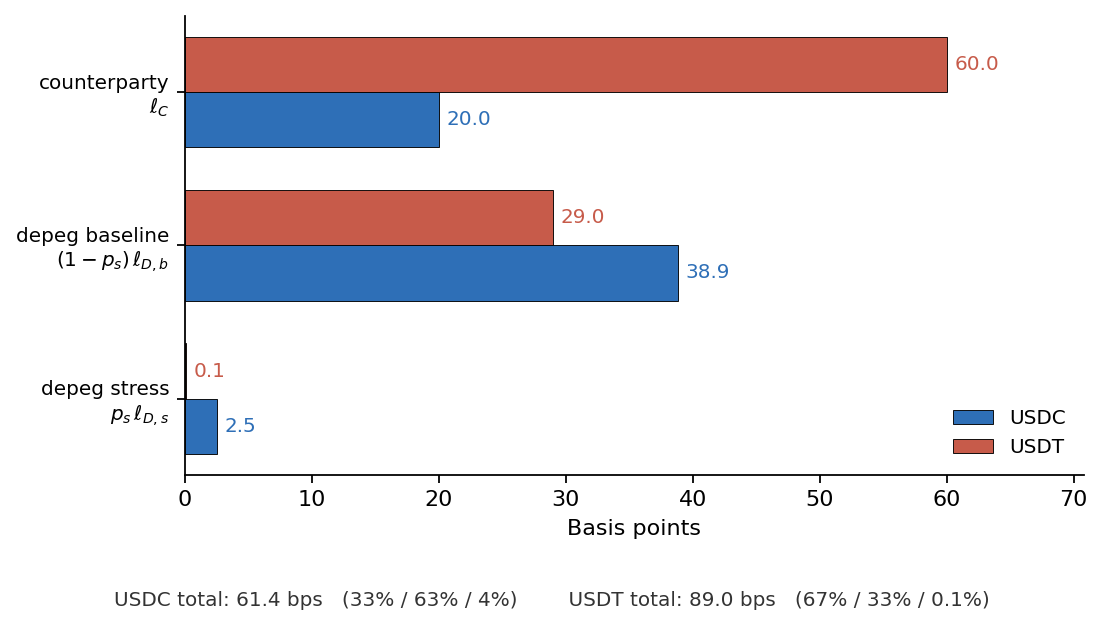
\includegraphics[width=\textwidth]{figures/fig_risk_decomposition.pdf}
\caption{Risk-premium decomposition for USDC and USDT, in basis points. USDC's 48.9\,bps total is depeg-dominant (54\% baseline depeg, 41\% counterparty, 5\% stress depeg); USDT's 71.2\,bps total is counterparty-dominant (84\% counterparty, 15\% baseline depeg, 0.4\% stress depeg). The same coordination machinery, calibrated to two issuers with structurally different reserves and secondary-market venues, returns inverted compositions.}\label{fig:risk_decomposition}
\end{figure}

\subsection{Mechanism check: depeg and redemption flows}\label{sub:mechanism_check}

The calibration imposes the model's depeg channel; we now check that channel against the data directly. The model's secondary price falls in unmet redemption pressure, convexly and the more steeply the thinner the market (Proposition~\ref{prop:reserves} and the price-impact function~\eqref{eq:psec}). We proxy redemption pressure by the daily net outflow of circulating supply (mint and burn, from DefiLlama) and the realised depeg by the daily maximum below-par deviation of the hourly secondary price (CryptoCompare), and regress one on the other, by issuer, over 2022--2026 (Table~\ref{tab:mechanism_check}).

\begin{table}[H]
\centering
\caption{Mechanism check. Daily depeg (basis points) on daily net redemption outflow (percent of circulating supply), redemption days only; HC1 $t$-statistics in parentheses.}\label{tab:mechanism_check}
\begin{tabular}{lrr}
\toprule
 & USDC & USDT \\
\midrule
Outflow slope (bps per 1\% outflow) & 27.5 \;(1.6) & 15.1 \;(2.1) \\
Quadratic term in outflow           & $+28.8$ \;(2.0) & $-7.0$ \;($-2.2$) \\
Shape of response                    & convex & concave \\
$R^2$ (quadratic)                    & 0.18 & 0.17 \\
Redemption days                      & 790 & 482 \\
\bottomrule
\end{tabular}
\end{table}

The model's sharpest prediction is a threshold: with unmet redemption $U = \max(D-R,0)$, the depeg should stay near zero until net redemptions exceed liquid reserves and then rise convexly. For USDC the data show exactly this kink. Estimating a breakpoint by grid search, the depeg is flat until net redemptions reach about $1.1\%$ of circulating supply and then rises at roughly 90 basis points per additional percentage point, nearly doubling the fit of a linear specification ($R^2$ of 0.17 against 0.08). For USDT no threshold is detected ($\hat\gamma \approx 0$), consistent with a deeper market that absorbs redemptions across the observed range. The same depth gap shows in the curvature of the unrestricted fit (Table~\ref{tab:mechanism_check}): the depeg rises with net redemptions for both issuers (15 to 28 basis points per percentage point), convexly for the thin USDC market and roughly linearly for the deep USDT one, the cross-issuer pattern the calibrated depth gap of Section~\ref{sub:not_homogeneous} predicts, recovered from the data without using the model. We read the check as supportive rather than decisive: the relationship is daily and noisy ($R^2$ between 0.08 and 0.18), the largest observed outflow is 3.6\%, so the deeply convex region where redemptions exceed liquid reserves is barely sampled, and depeg and outflow are jointly determined within a run, so the regression documents a conditional shape, not a causal effect.

These two episodes are plotted in Section~\ref{sec:risk_factors} (Figures~\ref{fig:svb_onchain} and~\ref{fig:terra_onchain}); the regression here is their quantitative counterpart. The realised depeg is severe when primary redemption is suspended, as for USDC over the SVB weekend, and mild when it is honoured at par, as for USDT over the Terra fallout.

\subsection{Mapping heterogeneity across the stablecoin universe}\label{sub:cross_section}

The two coins we calibrate, USDC and USDT, are the two largest fiat-backed stablecoins, together over 90\% of the segment. The rest of the universe varies along the two primitives the model identifies, reserve composition and secondary-market depth. Table~\ref{tab:cross_section} maps that variation: the realised depeg of seven fiat-backed stablecoins in the two systemic episodes, measured as the trough of the hourly secondary price.

\begin{table}[H]
\centering
\caption{Realised depeg of fiat-backed stablecoins in the two systemic episodes (trough of the hourly secondary price, basis points below par; CryptoCompare), ordered by the March 2023 depeg. The fractional-algorithmic FRAX is excluded as outside the fiat-backed scope.}\label{tab:cross_section}
\begin{tabular}{llrr}
\toprule
Stablecoin & Reserve profile & SVB 2023 & Terra 2022 \\
\midrule
DAI  & Crypto-collateralised, then majority USDC & 1082 & 24 \\
USDC & Treasuries and cash, exposed to SVB        & 978  & 16 \\
USDP & Treasuries and cash (Paxos), thin market   & 914  & 122 \\
GUSD & Treasuries and cash (Gemini), thin market  & 494  & 285 \\
TUSD & Mixed reserves, attestation-only           & 345  & 168 \\
BUSD & Treasuries (Paxos), segregated             & 17   & 36 \\
USDT & Mixed, offshore, attestation-only          & 4    & 249 \\
\bottomrule
\end{tabular}
\end{table}

The cross-section reproduces the reserve-quality comparative static of Proposition~\ref{prop:reserves} across issuers, and it does so with the sign reversing between episodes. In the March 2023 banking episode the depeg tracked exposure to the failed US bank: USDC, which held part of its cash reserve at Silicon Valley Bank, fell to 0.90, and DAI, then majority-collateralised by USDC, to 0.89, while the offshore USDT and the segregated-reserve BUSD held within twenty basis points of par; the smaller USDP, GUSD, and TUSD depegged by intermediate amounts, amplified by their thinner secondary markets. In the May 2022 Terra contagion the ordering inverts: the mixed-reserve, offshore USDT fell to 0.975 and the thin Gemini dollar to 0.97, while the clean, deep USDC barely moved. The two coins we calibrate therefore sit at opposite ends in opposite episodes, which is the inverted-composition result of Section~\ref{sec:identification} seen across the segment: a stablecoin's vulnerability is set by its reserve composition and secondary-market depth relative to the shock, not by the category label. USDC and USDT are the two poles of this map, and the calibrated premiums bracket the range the segment spans. Figure~\ref{fig:cross_section_map} plots the seven coins on the plane of the two episodes: USDC and USDT occupy opposite corners, while the remaining coins scatter between them according to their exposure to each shock, GUSD vulnerable to both and the segregated-reserve BUSD to neither.

\begin{figure}[H]
\centering
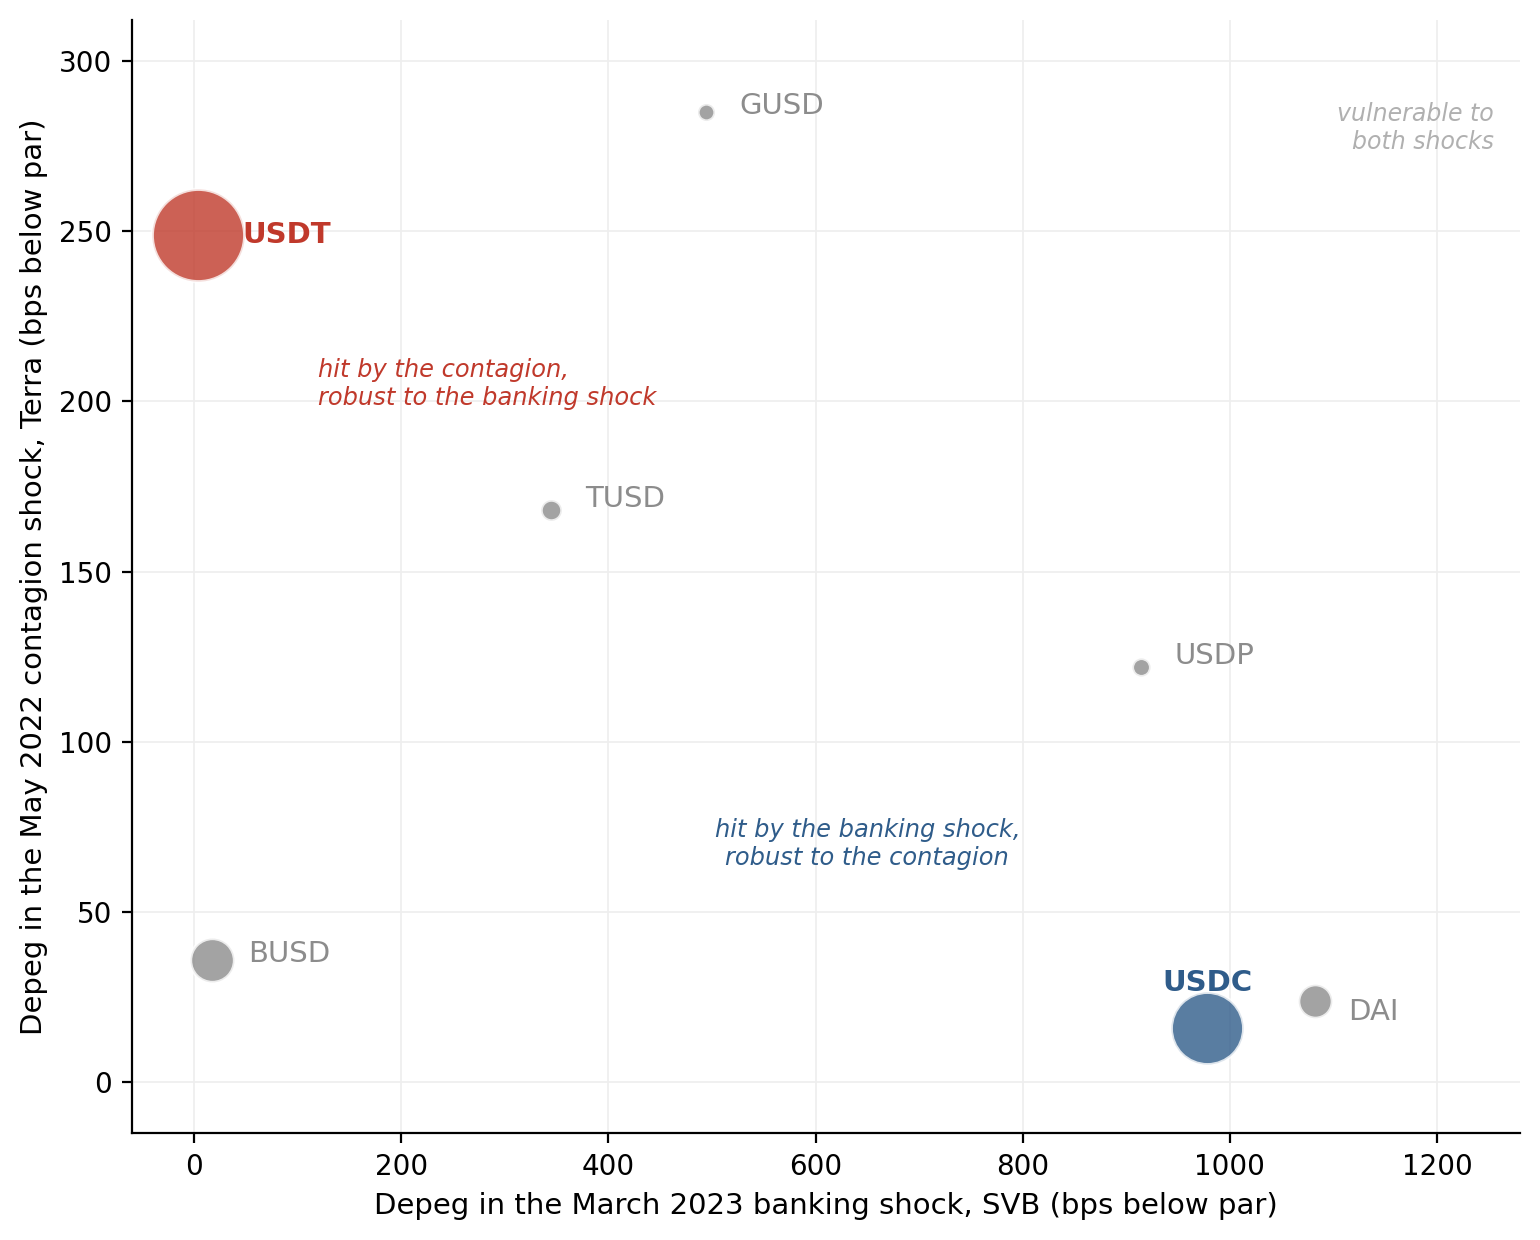
\includegraphics[width=0.92\textwidth]{figures/fig_cross_section_map.pdf}
\caption{Realised depeg of seven fiat-backed stablecoins in the two systemic episodes (trough of the hourly secondary price, basis points below par; CryptoCompare), plotted as the March 2023 banking-shock depeg against the May 2022 contagion-shock depeg. Bubble area is the coin's approximate peak circulating supply over 2022--2023, and USDC and USDT are highlighted as the two calibrated coins. A coin's vulnerability is shock-specific: USDC and DAI fall hard in the banking shock but not the contagion, USDT the reverse, so the two calibrated coins sit in opposite corners. Realised prices only; no model.}\label{fig:cross_section_map}
\end{figure}
